\begin{figure}[p]
\centering
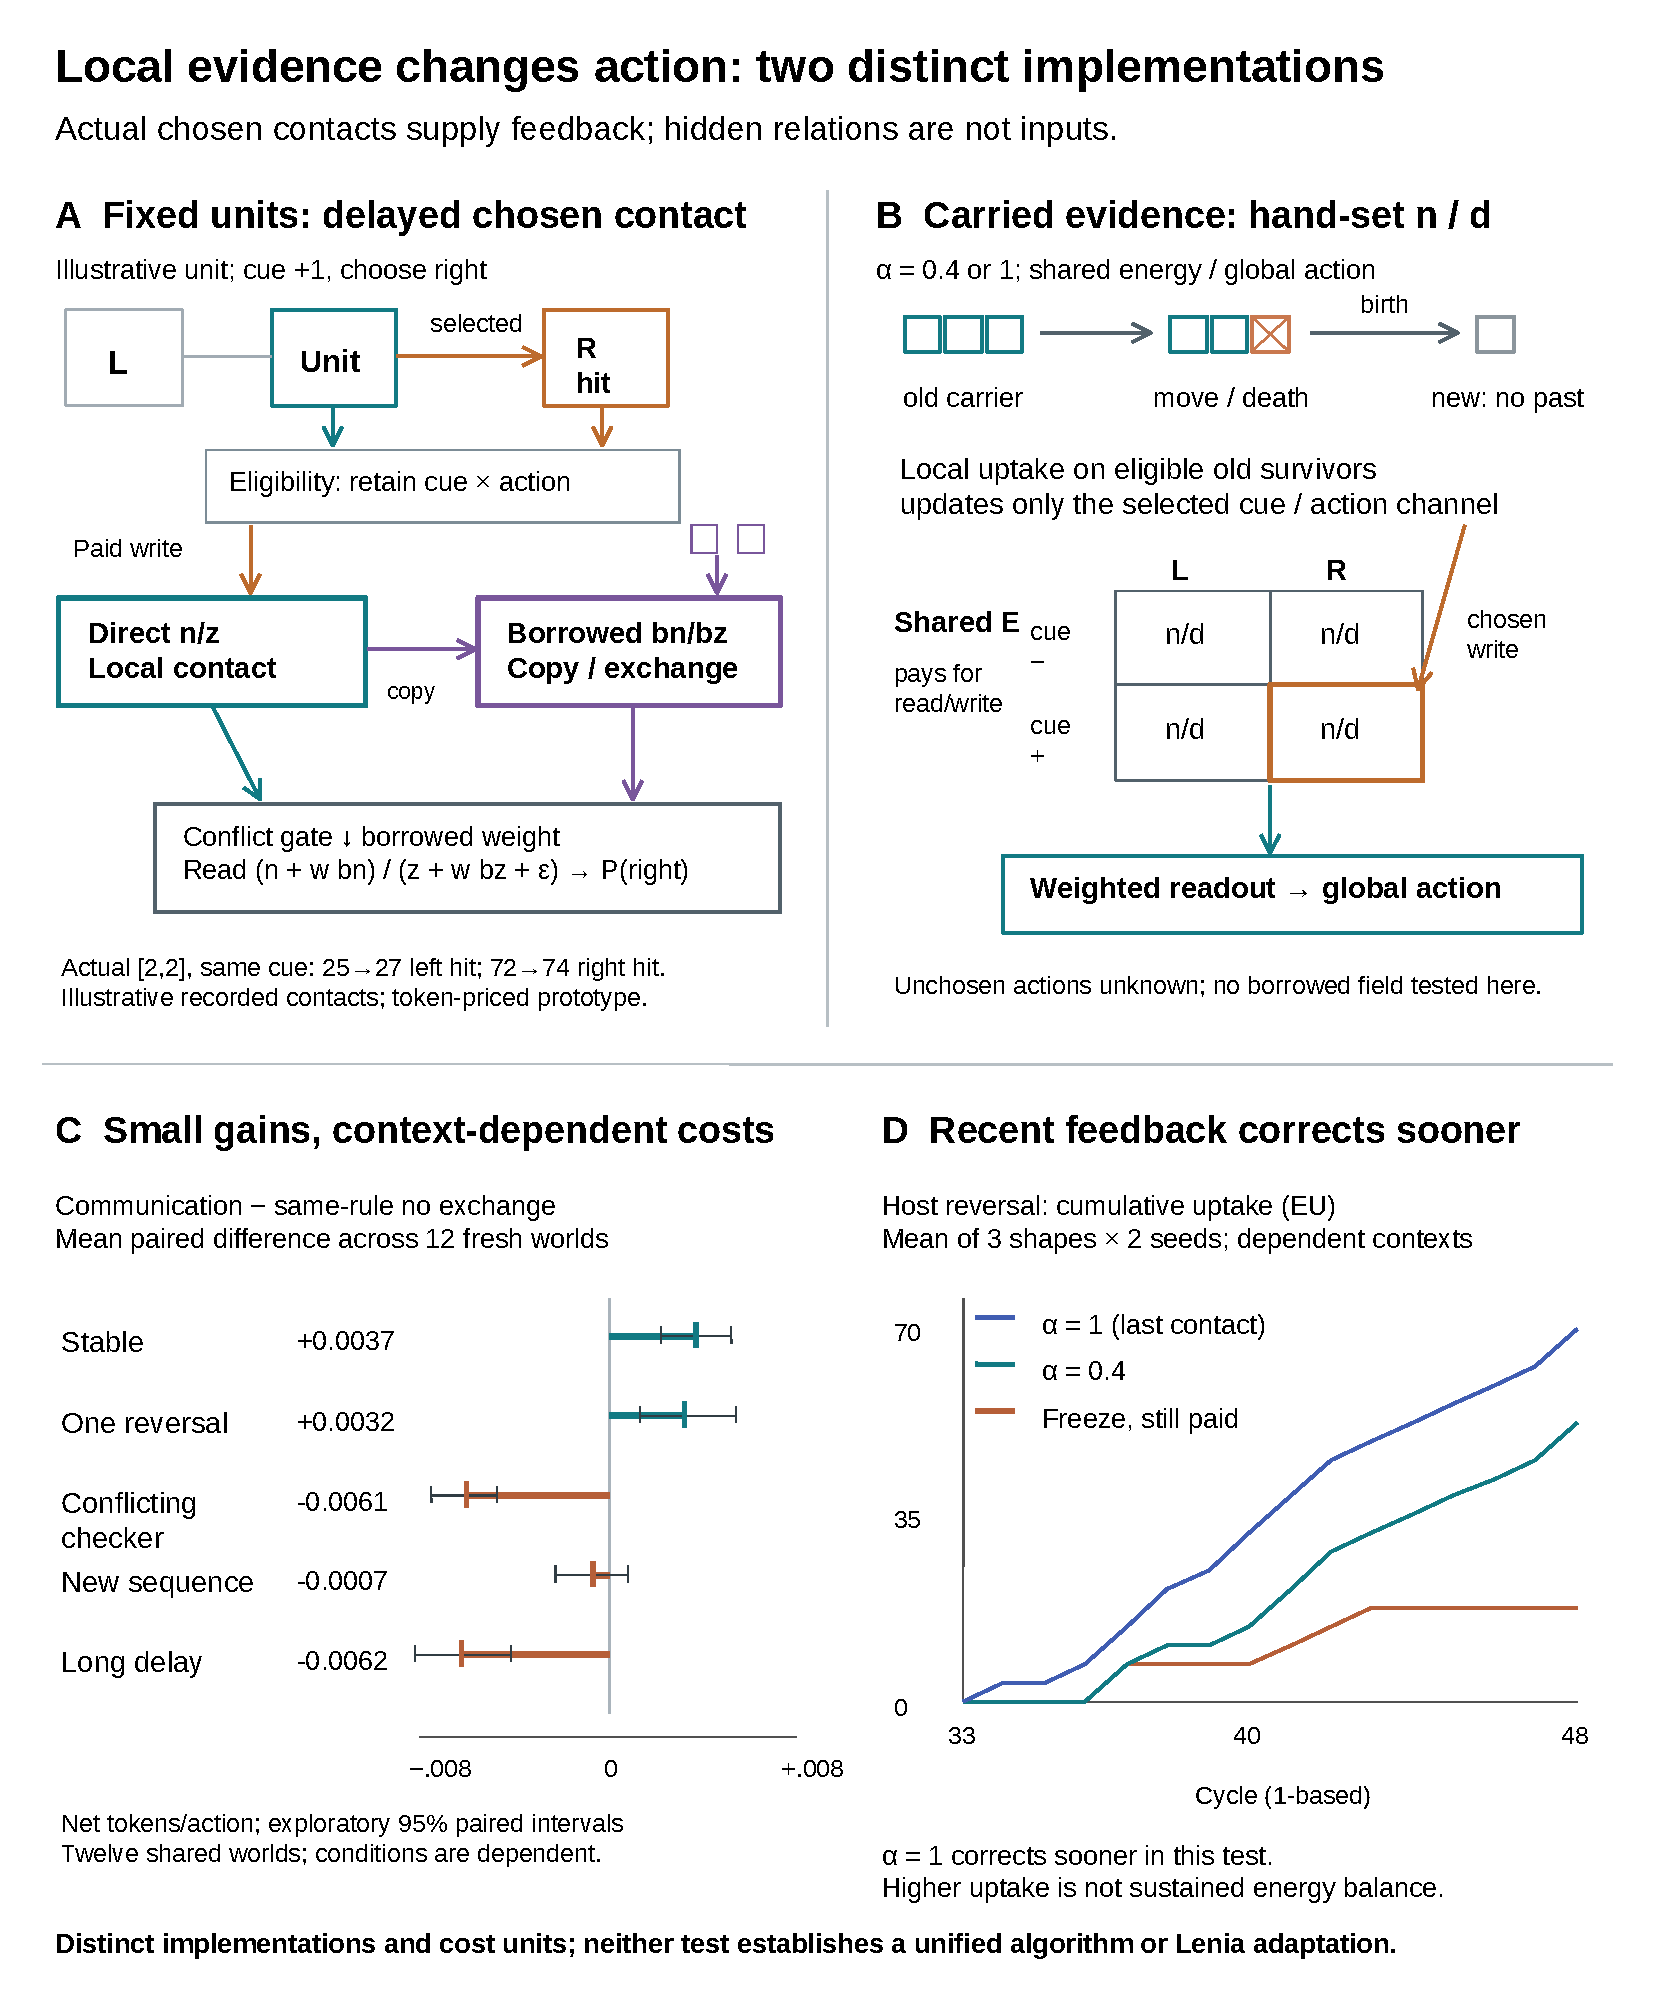
\includegraphics[width=\linewidth,height=0.79\textheight,keepaspectratio]{work/method_renewal/figures/local_evidence/local_evidence.pdf}
\captionsetup{font=footnotesize}
\caption{\textbf{Delayed local evidence connects encounters to later choices in two distinct implementations.}
\textbf{a}, Fixed contact units retain cue--action eligibility until an actual contact returns. Paid writes update direct evidence; a separate channel carries received estimates, whose influence is reduced by conflict with confident direct evidence. These units have token costs but no changing body.
\textbf{b}, A separate hand-set estimator attaches cue eligibility and uptake evidence to a moving density host. Surviving old carrier can write from local uptake; transport and death carry or remove stored state, while newborn tissue starts without past experience. A global readout and common energy reserve control movement and payment. This host does not implement the separated-message rule in \textbf{a}.
\textbf{c}, Communication minus no exchange at identical rule parameters: mean net-token differences across twelve paired world seeds. Intervals are exploratory 95\% paired bootstrap intervals. The same worlds recur across conditions.
\textbf{d}, Cumulative actual uptake after a new host reversal, averaged over three prescribed shapes sharing two environmental seeds. The latest-contact rate $\alpha=1$ corrects sooner than $\alpha=0.4$; paid freezing stops value writes. Increased uptake does not establish energy balance.}
\label{fig:local-evidence}
\end{figure}
